\begin{figure*}[bt!]
  \centering
  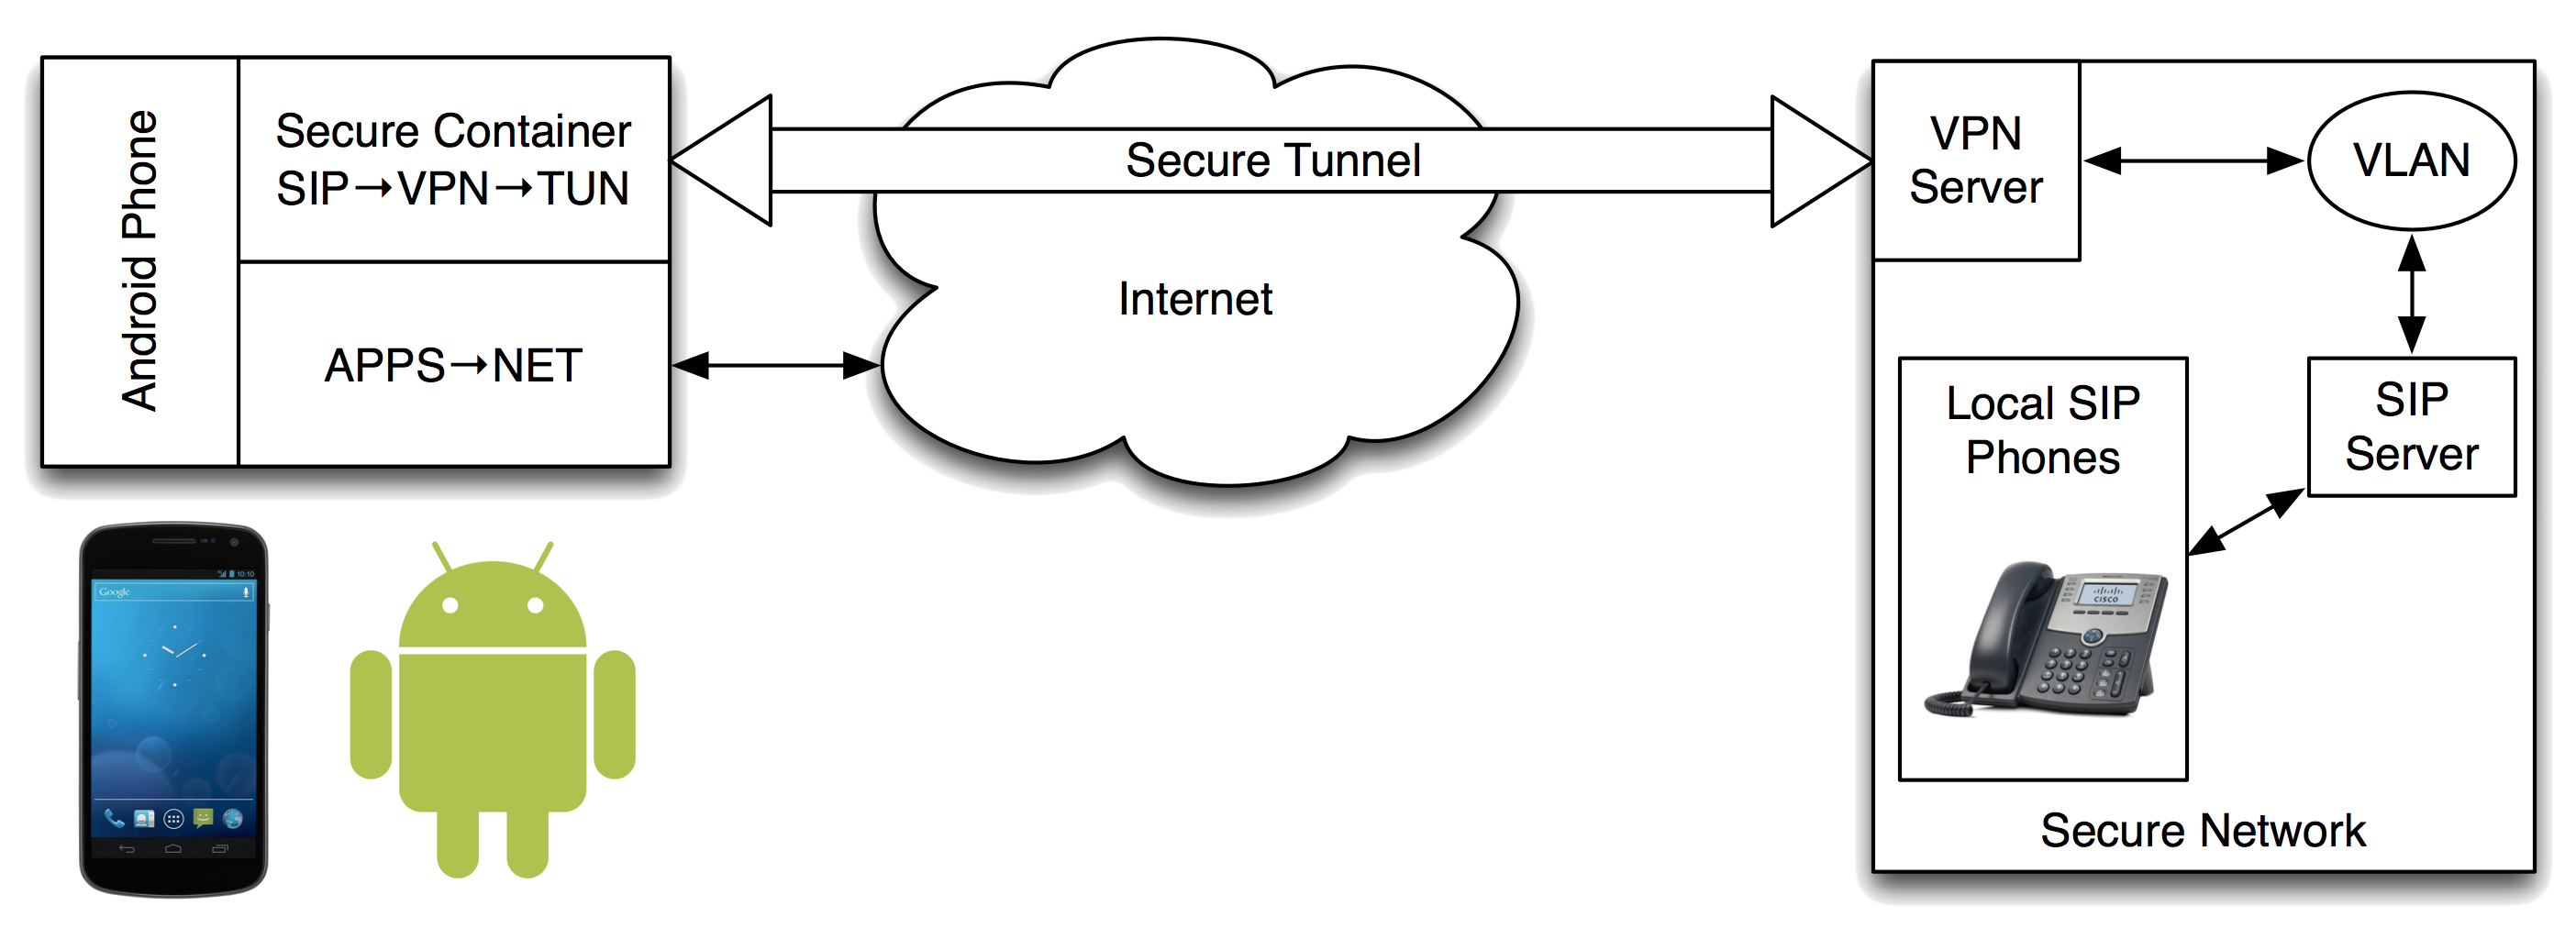
\includegraphics[width=.8\textwidth]{NetworkDiagram.png}
  \caption{Architectural layout}
  \label{fig:architecture}
\end{figure*}

Our approach was to first implement a secure \ac{voip} stack on the phone by creating a \ac{vpn} connection to a simulated enterprise.
We accomplished this by creating a virtual maching on Amazon's EC2 service which was running OpenVPN\footnote{\url{http://openvpn.net/}} and configured to only allow \ac{vpn} network traffic.
This virtual machine had one interface on the Internet and another on a \ac{lan} segment with no other connections to the Internet.
This \ac{lan} segment was where we placed users who were connected via \ac{vpn}.
We then created a virtual machine running FreePBX\footnote{\url{http://www.freepbx.org/}} to act as our \ac{sip} server, and attached it to the \ac{lan} segment as well.

After the servers were set up, we downloaded the Android source code from the \ac{aosp} for the android-4.0.3\_r1.1 branch.
We compiled our own kernel as well as created a system image with the standard Ice Cream Sandwich Operating System as well as the standard applications.
We then installed the OpenVPN client application and added our relevant keys.
Next we installed and configured Sipdroid\footnote{\url{http://code.google.com/p/sipdroid/}} to connect to our \ac{sip} server over the \ac{vpn} tunnel, as shown in Figure~\ref{fig:architecture}.

After that was configured and operating correctly, we obtained the \ac{seandroid} code for the same Android branch.
From this, we generated a new kernel and userspace, which included the \ac{selinux} enhancements.

We then reinstalled the OpenVPN and Sipdroid applications and booted the emulator with our new kernel and system image.
After we verified that the applications ran correctly, we modified the \verb=sepolicy= to label our \ac{vpn} interface, \verb=/dev/tun= with a type of \verb=tun_device= in the \verb=file_contexts= file.
We also added the OpenVPN application to the \verb=seapp_contexts= file so that we could create a new domain for the application.
We then regenerated our sytem image so that the new rules ensured that the device and application were properly labelled.

After booting the phone, we were then able to run our applications and obtain the \ac{avc} denial messages from the OpenVPN client attempting to manage the tunnel device.
We used those messages and the \verb=audit2allow= tool to generate an even more extensive policy which contained all of the actions OpenVPN was trying to perform, and added that to the \verb=app.te= file.

After regenerating the system image again, we no longer got any \ac{avc} denial messages when running the applications.
We must note here that we did not have to modify any characteristics of the Sipdroid application because its requests were made through \verb=binder= which strips any \ac{selinux} contexts from requests.
This effectively prevents any network based labelling and permissions.

